\documentclass[12pt,a4paper]{article}
\usepackage[utf8]{inputenc}
\usepackage[spanish]{babel}
%\usepackage{amsmath}
%\usepackage{amsfonts}
%\usepackage{amssymb}
\usepackage{hyperref}
\usepackage[pdftex]{graphicx}
\usepackage{fancyhdr}
\usepackage[font=small,labelfont=bf]{caption}
\pagestyle{fancy}
\lhead{\bfseries Redes de Datos -- Cloud Computing}
\rhead{}
%\chead{}
\newcommand{\HRule}{\rule{\linewidth}{0.5mm}}
\usepackage[left=2cm,right=2cm,top=2cm,bottom=2cm]{geometry}
\author{Ignacio Perez Laborda}

\hypersetup{pdfborder = {0 0 0}}

\begin{document}

\begin{titlepage}

\begin{center}

% Upper part of the page

\includegraphics[width=0.25\textwidth]{./logo_UB.png}\\[1cm] 

\textsc{\LARGE Universidad de Belgrano}\\[1.5cm]

\textsc{\Large Redes De Datos}\\[0.5cm]

%title
\HRule \\[0.4cm]
{ \huge \bfseries Trabajo Practico 2 -- Cloud Computing}\\[0.4cm]
\HRule \\[1.5cm]

% Author and supervisor
\begin{minipage}{0.4\textwidth}
\begin{flushleft} \large
\emph{Alumno:}\\
Ignacio \textsc{P\'erez Laborda}\\
Barbara \textsc{Mart\'inez}\\
\end{flushleft}
\end{minipage}
\begin{minipage}{0.4\textwidth}
\begin{flushright} \large
\emph{Matricula:} \\
502--10426\\
502--10402\\
\end{flushright}
\end{minipage}\\[1.5cm]

\vfill

%Bottom of the page
{\large \today}

\end{center}

\end{titlepage}


\tableofcontents

\listoffigures

\newpage

\section{¿Que es Cloud Computing?}

\subsection{Introducción}
Cuando se trata de un desarrollo, un problema muy común es la
infraestructura. Las grandes empresas tienen el capital
suficiente como para contratar a un ingeniero capaz de diseñar
una red de infraestructura adecuada a la información que se
maneja y a un personal que se encargue de administrar esa
red. Pero ¿Qué pasa cuando gente emprendedora que quiere empezar
un proyecto no tiene que almacenar la información suficiente
como para aprovechar, o no puede costear, un salón de
servidores? ¿O cuando se crea una aplicación que tiene un uso
temporal? ¿O se lanza una aplicación la cual no se sabe si
tendrá el suficiente éxito como para gastar fortunas en
infraestructura?. La respuesta es Cloud Computing, concepto
conocido también bajo los términos servicios en la nube. Es un
servicio de almacenamiento en el cual cualquier usuario puede
acceder a el sin las complicaciones que lleva montar
servidores, diseñar una topología y adecuar un ambiente para su
correcto desempeño. El usuario final no necesita tener
conocimientos avanzados de informática para utilizar estos
servicios ya que se puede presentar de muchas formas de cloud
computing, y quizás ni siquiera lo notemos, desde almacenamiento
de archivos que usamos cotidianamente y queremos tenerlos al
alcance siempre, hasta soporte de almacenamiento de datos para
aplicativos de proyectos caseros. Su versatilidad hace que hasta
también se adecúe al equipo y al tipo de plataforma en el cual
nos estemos conectando para visualizar nuestra información,
tablets, equipos de escritorio, celulares, entre otros.\par

La computación en la nube son servidores desde internet
encargados de atender las peticiones en cualquier momento. Se
puede tener acceso a su información o servicio, mediante una
conexión a internet desde cualquier dispositivo móvil o fijo
ubicado en cualquier lugar. Sirven a sus usuarios desde varios
proveedores de alojamiento repartidos frecuentemente por todo el
mundo. Esta medida reduce los costes, garantiza un mejor tiempo
de actividad y que los sitios web sean invulnerables. Es un nuevo
modelo de prestaciones que hasta le permite al usuario tener un
catálogo online de todos los servicios que ofrece, aumentando
mas una de sus cualidades mas importantes que es la
flexibilidad. Esto genera beneficios tanto para los proveedores,
que pueden ofrecer, de forma más rápida y eficiente, un mayor
número de servicios, como para los usuarios que tienen la
posibilidad de acceder a ellos, disfrutando de la
``transparencia'' e inmediatez del sistema y de un modelo de pago
por consumo, así el consumidor puede controlar sus gastos.\par 
Se incorporan conceptos como  el ``software como servicio'' y otros
mas recientes que son tendencias tecnológicas que tienen en
común el que confían en Internet para satisfacer las necesidades
de cómputo de los usuarios.


\begin{figure}[h!]
 \centering
 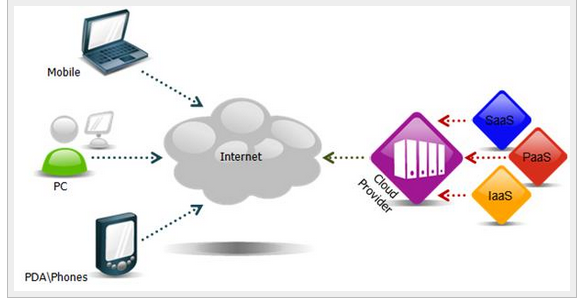
\includegraphics[width=0.71\textwidth]{cc_def.png}
\caption[Ruta de datos]{Ruta de la información en cloud
computing}
\end{figure}

\par
\subsection{Características importantes de Cloud Computing}

Para obtener la eficiencia que se conoce hoy en día, cloud
computing atiende a una serie de características básicas que las
difieren de otros servicios de almacenamiento:
\begin {itemize}
\item \textbf{Flexibilidad en la elección de aplicaciones:} El
usuario puede decidir en todo momento qué aplicaciones usar y
elegir entre aquellas que son gratuitas y las que no lo son. En
el caso de las aplicaciones de pago, el coste irá en función de
diversas variables, como el servicio contratado, el tiempo que
se ha usado ese servicio, el volumen de tráfico de datos
utilizado, etc.
\item \textbf{Accesibilidad:} Se encuentra una disponibilidad
completa de las aplicaciones en cloud computing y libres para el
usuario. El rango es muy amplio y varía desde el uso de PCs hasta
portátiles y móviles.

\item \textbf{Asignación de recursos en modo multiusuario:} A
diferencia de las aplicaciones de software tradicionales, en el
cloud computing el proveedor tiene una única aplicación que abre
a todos los usuarios que desean utilizarla, estableciendo unos
recursos de acceso y prestaciones distintos para cada usuario.
Al ser aplicaciones multiusuario, puede hacer miles de
internautas utilizando la misma herramienta a la vez, cada uno
con las mismas o distintas prestaciones.

\item \textbf{Elasticidad y escalabilidad:} Las aplicaciones en
cloud son totalmente elásticas en cuanto a su rapidez de
implementación y adaptabilidad. Además, son totalmente
escalables, es decir, hoy podemos estar utilizando solo un 10
\% del total de la aplicación y mañana podemos acceder al 80
\% de la misma con total normalidad y rapidez, con tan solo
comunicarlo a nuestro proveedor y modificar nuestra tarifa de
suscripción.
 
\item \textbf{Supervisión del servicio:} Los sistemas en cloud
controlan y optimizan el uso de los recursos de manera
automática, por lo que el uso de estos puede seguirse,
controlarse y notificarse, lo que aporta transparencia tanto
para el proveedor como para el consumidor del servicio
utilizado.
 
\item \textbf{Seguridad:} Los datos, cuando están en aplicaciones
en cloud, se alojan en DATA CENTERS, empresas específicamente
dedicadas a la custodia y salvaguarda de datos de empresas de
todo tipo. Son empresas que cuentan con todas las medidas de
seguridad necesarias, tanto físicas como de software, de forma
que no haya jamás una pérdida de información ni de integridad de
los datos.
\end{itemize}

\begin{figure}[h!]
 \centering
 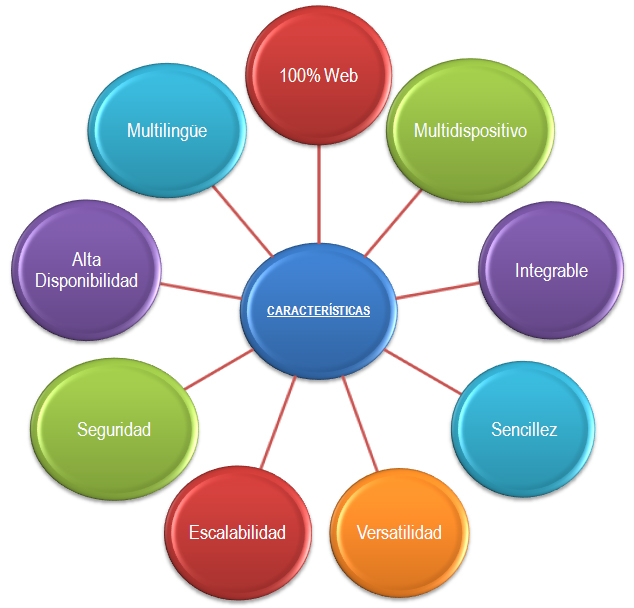
\includegraphics[width=0.61\textwidth]{Caracteristicas2.png}
 \caption[Características]{Características del cloud computing}
\end{figure} 

\subsection{Las Ventajas de Cloud Computing}

\begin {itemize}
\item \textbf{Mejora en la economía} El poder aumentar la
capacidad de producción con la menor cantidad de
personas. Asegura un mayor rendimiento costo-beneficio.

\item \textbf{Reducir el gasto en infraestructura tecnológica}
Se otorga un fácil acceso a la información con un gasto fijo y
mínimo por adelantado.

\item \textbf{Globalización de la fuerza de trabajo} Todas las
personas pueden acceder a la nube siempre y cuando tengan
conexión a internet.
\item \textbf{Optimización de los procesos} Hacer mayor trabajo
en menos tiempo.
 
\item \textbf{Reducir los costos de capital} No hay necesidad de
gastar dinero en hardware, software o licencias.
 
\item \textbf{Mejora la accesibilidad} Acceso en cualquier
momento y en cualquier lugar.
  
\item \textbf{Supervisar los proyectos con mayor eficacia}
Facilidad para supervisar el tiempo y costo de los proyectos y
presupuestarlos.
 
\item \textbf{ Menos entrenamiento de personal} No hay que
gastar recursos en capacitación de personal ya que solo se
requieren conocimientos mínimos de software.
  
\item \textbf{ Mejorar la flexibilidad} Puede cambiar de
capacidad fácilmente y adaptarlo rápidamente a las necesidades
del usuario.
    
\end{itemize}


\begin{figure}[h!]
 \centering
 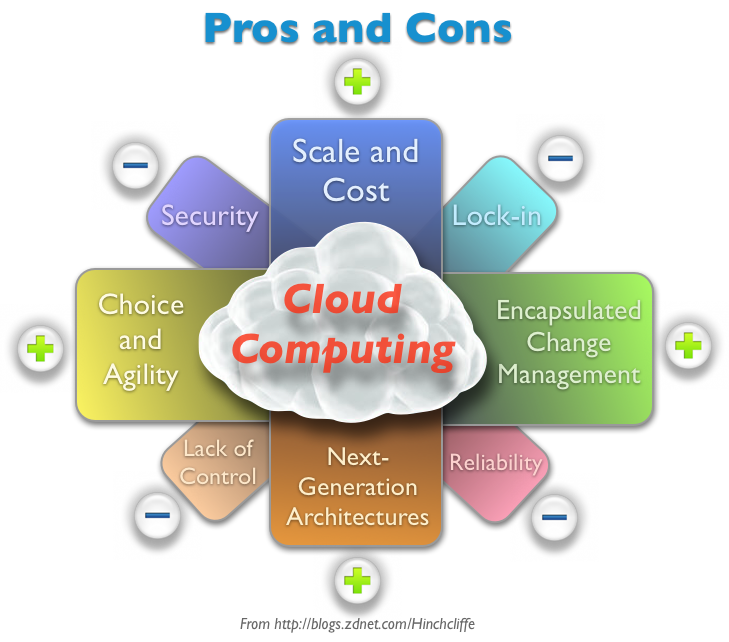
\includegraphics[width=0.54\textwidth]{cc_pros.png}
\caption[Pros Cloud Computing]{Esquema de ventajas y desventajas de cloud computing}
\end{figure}\par


\section{Distintos Servicios de Cloud Computing}

\begin{figure}[h!]
 \centering
 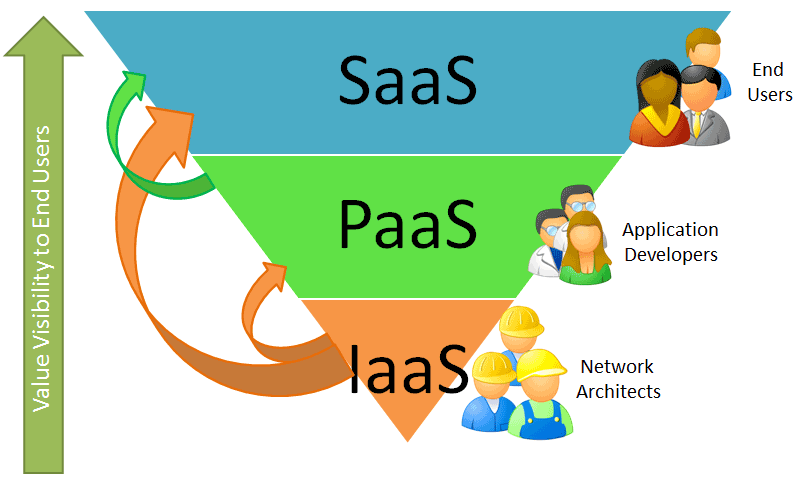
\includegraphics[width=0.79\textwidth]{SaStoIaS.png}
\caption[Servicios de Cloud Computing]{Servicios de cloud computing}
\end{figure}

\subsection{SaaS -- Software as a Service}
En el sistema tradicional un cliente compra o manda a hacer una aplicación y 
este es dueño de una licencia, se le entrega físicamente el código fuente o
el binario listo a ser ejecutado de esa manera por cada instancia del 
programa hacia falta tener una licencia. Además la disponibilidad de los 
programas y la instalación corrían a cargo del cliente implicando mayores 
gastos. También muchas veces se pagaba por un software no muy adaptado a las 
necesidades especificas sino a términos mas generales, la personalizacion del 
software se volvía muy cara y dificultosa.\par
Saas es aquella aplicación ofrecida por su creador (ISV) a través de internet 
para su uso o utilización por varios clientes manteniendo la privacidad de 
sus datos y la personalización de la aplicación. El usuario paga por el uso, 
por la infraestructura necesaria (CPD, máquinas de computación, de 
almacenamiento, de seguridad,etc) para el correcto funcionamiento de la 
aplicación y por el mantenimiento (nuevas versiones, corrección de bugs, 
almacenamiento necesario,etc) de la infraestructura y aplicación.\par
El hecho de que se acceda a la aplicación a través de internet no quiere 
decir que se haga a través de navegador pero la utilidad más interesante de 
este tipo de aplicaciones es que se haga a través del navegador y no requiera 
instalación en las máquinas de los usuarios de la aplicación. En esta 
comparativa entre saas y el software instalado in-house  podemos sacar 
conclusiones de los beneficios del saas.\par
El modelo Saas establece estas características:
\begin{itemize}

\item \textbf{Configuración y customizacion: }
Las aplicaciones Saas soportan lo que tradicionalmente se conoce como 
personalizacion de aplicaciones. En este caso un cliente puede alterar un 
conjunto de parámetros de configuración que afectan el look and feel y cierta 
funcionalidad. De esta manera cada cliente puede tener su propia 
configuración.

\item \textbf{Actualizaciones rápidas: }
Las aplicaciones Saas son actualizadas frecuentemente. Esto se logra por el 
hecho de que la aplicación se encuentra hosteada en un solo lugar y la 
actualización es decidía por el proveedor no los clientes.Esto se ve 
acentuado por las metodologías agiles las cuales permiten lanzamientos en 
menor tiempo. 

\item \textbf{Uso de protocolos abiertos: }
Dados que estos sistemas no acceden a las compañías y no necesariamente 
interactúan con otros sistemas se aseguran de operar con estándares abiertos
de esta manera se pueden interconectar con una mayor cantidad de clientes y 
ofrecer el servicio a mas mercados.

\end{itemize}

Las ventajas son:
\begin{enumerate}

\item No es necesario que el cliente cuente con un área especializada de 
soporte para el sistema, por lo que se reducen sus costes y riesgo de 
inversión.
\item La responsabilidad de la operación recae en la empresa IT. Esto 
significa que la garantía de disponibilidad de la aplicación y su correcta 
funcionalidad, es parte del servicio que da la compañía proveedora del 
software.
\item La empresa IT no desatiende al cliente. El servicio y atención continua 
del proveedor al cliente es necesaria para que este último siga pagando el 
servicio.
\item La empresa IT provee los medios seguros de acceso en los entornos de la 
aplicación. Si una empresa IT quiere dar SaaS en su cartera de productos, 
debe ofrecer accesos seguros para que no se infiltren datos privados en la 
red pública.
\item No es necesaria la compra de una licencia para utilizar el software, 
sino el pago de un alquiler o renta por el uso del software. Aunque también 
se dan casos particulares donde el servicio es totalmente gratuito, como por 
ejemplo en el servicio de blogs que brindan diferentes compañías: Wordpress, 
Blogger, etc; es decir, se cuenta con el servicio, se puede acceder 
libremente, se garantiza usabilidad y actualidad, pero no se paga por el 
servicio.
\item Se le permite al cliente completa flexibilidad en el uso de los 
sistemas operativos de su preferencia, o al cual pueda tener acceso.

\end{enumerate}

Mientras que las desventajas son:
\begin{enumerate}

\item La persona usuaria no tiene acceso directo a sus contenidos, ya que 
están guardados en un lugar remoto, y en caso de no contar con mecanismos de 
cifrado y control disminuye el índice de privacidad, control y seguridad que 
ello supone, ya que la compañía TI podría consultarlos.
\item El usuario no tiene acceso al programa, por lo cual no puede hacer 
modificaciones (dependiendo de la modalidad del contrato de servicios que 
tenga con la compañía TI).
\item Al estar el servicio y el programa dependientes de la misma empresa, no 
permite al usuario migrar a otro servicio utilizando el mismo programa 
(dependiendo de la modalidad del contrato de servicios con la compañía de 
TI).
\item Si el servicio de Internet no está disponible por parte del ISP, el 
usuario no tendrá acceso al programa, por lo que sus operaciones se verán 
afectadas hasta que dicho servicio se restablezca.

\end{enumerate}

\subsection{PaaS -- Platform as a service}
Una vez que tenemos desarrolladas nuestras aplicaciones para la nube estas deben hacer uso de otras 
plataformas, como servidores HTTP, servidores de aplicaciones, bases de datos, colas de mensaje, etc.
Tradicionalmente nosotros debíamos de proveer también de dichas aplicaciones, pero con la llegada de
la nube ahora tenemos proveedores de dichos servicios, los llamados PaaS (Platform as a service).\par
PaaS incluye todas las facilidades al programador para prototipar, análizar, desarrollar, testear, 
documentar y poner en marcha aplicaciones todo en un sólo proceso. Paas da servicio de integración de 
la base de datos, seguridad, escalabilidad, almacenaje, copias de seguridad, versioning, y facilidad 
para colaborar en la comunidad. Aquí si nuestra aplicaciones necesitas de mas recursos estos pueden 
ser alocados por el proveedor de manera automática y se suele cobrar, por recursos utilizados u horas 
de uso.\par 
Algunas características:
\begin{enumerate}

\item \textbf{Facilidad de uso: }
Las plataformas PaaS son comúnmente diseñadas alrededor de las preferencias de los desarrolladores 
para maximizar la productividad.

\item \textbf{Simplicidad: }
PaaS permite enfocar los recursos en la adición de valor agregado removiendo las tareas no 
diferenciadoras asociadas a los proyectos, como proveer y manejar los ambientes

\item \textbf{Automatización: }
Las plataformas PaaS realizan un uso muy intensivo de la automatización para eliminar las tareas 
repetitivas que no agregan valor, para así dejar a los desarrolladores enfocarse en las tareas de 
diferenciación del producto.

\item \textbf{Arquitectura multi-usuario : }
PaaS intenta soportar típicamente aplicaciones con muchos usuarios concurrentemente, proveyendo
administradores de concurrencia, escalabilidad, fail-over y seguridad.

\item \textbf{Integracion con web services y bases de datos: }
El soporte a interfaces SOAP y REST permite crear composiciones de multiples servicios web, aveces 
llamados ``mashups".

\end{enumerate}

\begin{figure}[h!]
 \centering
 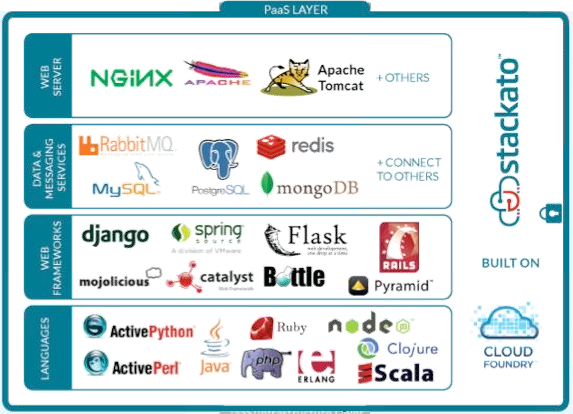
\includegraphics[width=0.98\textwidth]{stackAto.png}
\caption[Stack PaaS]{Stack PaaS}
\end{figure}

\subsection{IaaS -- Infrastructure as a service}
Con la popularización de la virtualizacion, una técnica que nos permite poder correr sistemas 
operativos completos como si fueran aplicaciones dentro de nuestra maquina real, se ha permito
multiplicar y bajar los costos de los servidores. Ahora a partir de una sola maquina real se puede 
tener muchas maquinas virtuales y a cada una asignarle una tarea. Dicha maquina virtual puede ser 
clonada o transportada a otra maquina real. Actualmente existen muchas técnicas para lograrla, pero 
todas nos permiten realizar lo mismo. Esto es muy importante porque se ha bajado mucho el precio de 
los servidores dedicados lo cual nos lleva a la Infraestructura como servicio (IaaS).\par
Entonces ahora se puede virtualizar y ofrecer todas las herramientas de la infraestructura, como
almacenamiento, poder de computo, infraestructura de redes, etc como un servicio a terceros. Por 
ejemplo en vez de comprar microprocesadores mas rápidos o mas módulos de memoria RAM, podemos 
adquirir mas poder de procesamiento y solicitar mas memoria, la administración de esta y su 
implementación no corre por nuestra cuenta, además de que los cambios suelen ser instantáneos. Esto 
permite a las empresas no tener un área grande dedicada a la infraestructura, con sus consiguientes 
gastos en mantenimiento y escalabilidad. Todo eso queda tercerizado en la empresa a quien contratemos 
el servicio. Esto permite bajar los precios y especializar a las empresas en un solo rubro. Otra gran 
ventaja que presenta dicho modelo es que solo se paga por lo q se utiliza, no hace falta tener discos 
grandes o memoria de sobra, solo lo necesario para que los sistemas funcionen.\par
Entre las ventajas de IaaS podemos encontrar:\\

\begin{enumerate}

\item \textbf{IaaS es flexible.} Si hoy necesita un pequeño servidor y el mes que viene uno grande. 
Si descubre que el servidor que acaba de adquirir es pequeño para el software que va a instalar, 
podrá hacer crecer o encoger su infraestructura según sus necesidades.

\item \textbf{IaaS es rápido.} Desde que decida tener un nuevo servidor, hasta que lo tiene 
disponible, el tiempo se cuenta en minutos.

\item \textbf{IaaS no tiene coste oculto.} No hay electricidad, refrigeración, espacio ocupado, 
control de accesos. Todos esos costes que deberíamos de sumar a la propiedad de infraestructura, 
desaparecen. Simplemente tendrá un gasto mensual por el uso que haga de la infraestructura.

\item \textbf{IaaS es fiable.} Más que tener los servidores en sus instalaciones. Las 
infraestructuras se alojan en CPD’s de alto nivel, que cuentan con todas las medidas necesarias para 
estar siempre operativos. Comunicaciones y energía redundante, sistemas anti-incendio, control de 
accesos, etc. Niveles de disponibilidad de un 99,95 \%.

\end{enumerate}

Como ejemplo tomaremos a uno de los prestadores de servicio mas importante en el ambiente, Amazon y 
su servicio Amazon Elastic Compute Cloud (EC2). Aquí se pueden solicitar instancias que son la unidad 
en la que se vende el servicio, representarían a un servidor ``real". Las cuales existen en varias 
tipos de combinaciones entre poder de computo, memoria RAM, disco rígido y capacidades de I/O de red.
Estas se pueden adquirir con tarifas planas, por casos puntuales o en demanda y van desde pequeñas 
instancias a grande, el sistema operativo también puede ser elegido habiendo distintos precios. 
Dentro de dichas ``maquinas" uno puede correr las aplicaciones que desee y si estas necesitan en 
ciertos casos mas recursos estos también se puede solicitar puntualmente.

\begin{figure}[h!]
 \centering
 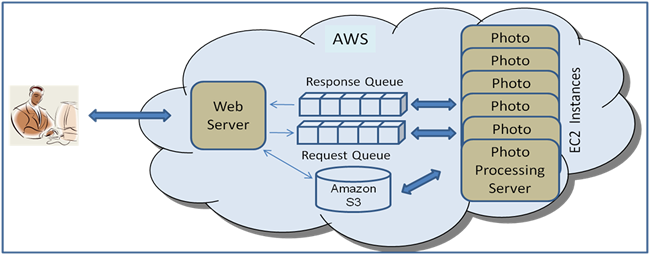
\includegraphics[width=1\textwidth]{159_madhu.png}
\caption[Amazon EC2]{Amazon EC2}
\end{figure}

\section{Seguridad en Cloud Computing}
Cloud computing requiere un modelo de
seguridad que reconcilie la escalabilidad y la tenencia
múltiple con la necesidad de confianza. A medida que las
empresas trasladan sus ambientes informáticos con las
identidades, la información y la infraestructura a la nube,
deben estar dispuestas a renunciar a cierto nivel de control.
Para hacerlo, deben confiar en los sistemas y los
proveedores de nubes, y verificar los procesos y los eventos
de nubes. Entre los componentes básicos importantes de la
confianza y de las relaciones de verificación, se incluyen el
control de acceso, la seguridad de los datos, el
cumplimiento de normas y la administración de eventos;
todos ellos son elementos de seguridad bien comprendidos
por los departamentos de TI actuales, implementados con
productos y tecnologías existentes, y extensibles a la nube.

\subsection{Seguridad de la identidad}
La administración de identidades end-to-end, los servicios
de autenticación de otros fabricantes y la identidad federada
se convertirán en un elemento clave de la seguridad de la
nube. La seguridad de la identidad preserva la integridad y la
confidencialidad de los datos y las aplicaciones, a la vez que
ofrece acceso de disponibilidad inmediata a los usuarios
adecuados. El soporte para estas capacidades de
administración de identidades de usuarios y componentes

de la infraestructura será un requerimiento importante para
cloud computing, y la identidad deberá administrarse de
manera que cree confianza. Se requerirá.
\begin{itemize}

\item Autenticación sólida: cloud computing debe ir más
allá de la autenticación débil de nombres de usuario y
contraseñas si pretende brindar soporte a la empresa.
Esto significa adoptar técnicas y tecnologías que ya
son estándar en el área de TI empresarial, como la
autenticación sólida (autenticación de múltiples
factores con tecnología de contraseña de un solo uso),
la federación dentro de las empresas y entre estas, y la
autenticación basada en riesgos que mide el historial de
comportamiento, el contexto actual y otros factores que
permiten evaluar el nivel de riesgo de la solicitud de un
usuario. Niveles adicionales de autenticación serán
fundamentales para cumplir con los acuerdos de nivel
de servicio de seguridad; y el uso de un modelo de
autenticación basado en riesgos que sea transparente
en gran medida para los usuarios reducirá la necesidad
de una federación más amplia de controles de acceso.

\item Autorización más granular: la autorización puede
ser general en una empresa o, incluso, en una nube
privada. No obstante, para manejar datos delicados y
requerimientos de cumplimiento de normas, las nubes
públicas necesitarán capacidades de autorización
granular (como controles basados en funciones e IRM)
que puedan ser persistentes en toda la infraestructura
de nube y el ciclo de vida de los datos.

\end{itemize}

\begin{figure}[h!]
 \centering
 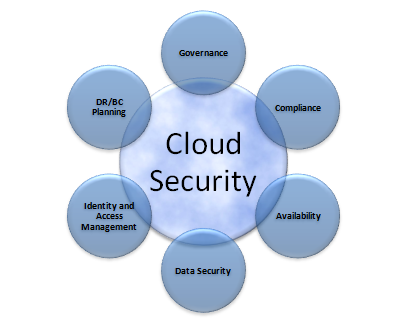
\includegraphics[width=0.77\textwidth]{cloudsecurity1220.png}
\caption[Seguridad en Cloud]{Seguridad en cloud computing}
\end{figure}\par

\subsection{Seguridad de la información}
En el data center tradicional, los controles sobre el acceso
físico, el acceso a hardware y software, y los controles de
identidad se combinan para la protección de los datos. En la
nube, esa barrera de protección que garantiza la seguridad
de la infraestructura se disipa. Para compensar, la seguridad
deberá estar centrada en la información. Los datos necesitan
que su propia seguridad se traslade con ellos y los proteja.
Se requerirá.

\begin{itemize}

\item \textbf{Aislamiento de datos:} en situaciones de tenencia
múltiple, será necesario mantener los datos de manera
segura para protegerlos cuando varios clientes usen
recursos compartidos. La virtualización, la encriptación
y el control de acceso serán excelentes herramientas
que permitirán distintos grados de separación entre
las corporaciones, las comunidades de interés y los
usuarios. En el futuro cercano, el aislamiento de datos
será más importante y ejecutable para IAAS de lo que
quizá será para PAAS y SAAS.

\item \textbf{Seguridad de datos más granular:} a medida que
la confidencialidad de la información aumenta, la
granularidad de la implementación de la clasificación
de los datos debe aumentar. En los ambientes de data
center actuales, la granularidad del control de acceso
basado en funciones a nivel de grupos de usuarios o
unidades de negocios es aceptable en la mayoría de
los casos porque la información permanece dentro del
control de la empresa. Para la información en la nube,
los datos delicados requerirán seguridad a nivel de
archivos, campos o incluso bloques para satisfacer las
demandas de seguridad y cumplimiento de normas.

\item \textbf{Seguridad de datos coherente:} habrá una necesidad
evidente de contar con protección de contenido basada
en políticas para satisfacer las necesidades propias de la
empresa y las directivas de políticas reglamentarias. Para
algunas categorías de datos, la seguridad centrada en la
información necesitará encriptación en transmisión y en
reposo, además de administración en la nube y en todo
el ciclo de vida de los datos.

\item \textbf{Clasificación eficaz de datos:} cloud computing impone
un intercambio de recursos entre el alto rendimiento
y los requerimientos de mayor seguridad sólida. La
clasificación de los datos es una herramienta fundamental
para equilibrar esa ecuación. Las empresas necesitarán
saber qué datos son importantes y dónde están ubicados
como requerimiento previo para tomar decisiones
relacionadas con el costo/beneficio del rendimiento,
además de garantizar el enfoque en las áreas más
críticas para los procedimientos de prevención de
pérdida de datos.

\item \textbf{Administración de derechos de información:} se suele
tratar a IRM como un componente de identidad, una
forma de establecer controles generales sobre qué
usuarios tienen acceso a los datos. No obstante, la
seguridad centrada en los datos más granular requiere
que las políticas y los mecanismos de control sobre el
almacenamiento y el uso de información estén asociados
directamente con la información en sí.

\item \textbf{Buen manejo y control y cumplimiento de normas:}
un requerimiento clave del buen manejo y control y el
cumplimiento de normas de la información corporativa
es la creación de información de administración y
validación; se realiza el monitoreo y la auditoría del
estado de seguridad de la información con capacidades
de registro. Aquí, no solo es importante documentar
el acceso y la denegación de acceso a los datos,
sino también garantizar que los sistemas de TI estén
configurados para cumplir con las especificaciones de
seguridad y no se hayan alterado. La expansión de las
políticas de retención para el cumplimiento de normas
y políticas de datos también se convertirá en una
capacidad esencial de la nube. Básicamente, las
infraestructuras de cloud computing deben tener la
capacidad de verificar que se administren los datos
según las reglamentaciones locales e internacionales
correspondientes (como PCI y HIPAA) con controles
adecuados, recopilación de logs y creación de informes.

\subsection{Seguridad de la infraestructura}
La infraestructura base para una nube debe ser
inherentemente segura, ya sea una nube privada o pública,
o un servicio SAAS, PAAS o IAAS. Se requerirá.
\item \textbf{Seguridad inherente de componentes:} la nube debe
estar diseñada para ser segura, creada con componentes
inherentemente seguros, implementada y aprovisionada
de manera segura con interfaces sólidas a otros
componentes y, finalmente, soportada de manera
segura con procesos de evaluación de vulnerabilidades
y administración de cambios que producen información
de administración y seguridades de nivel de servicio que
crean confianza. Para estos componentes implementados
de manera flexible, la identificación mediante la huella
digital del dispositivo para garantizar la seguridad de la
configuración y el estado también será un elemento de
seguridad importante, al igual que lo es para los datos
y las identidades en sí.
\item \textbf{Seguridad de interfaz más granular:} los puntos en
el sistema en los que se presentan intervenciones
(usuario a red, servidor a aplicación) requieren políticas
y controles de seguridad granulares que garanticen
consistencia y responsabilidad. Aquí, el sistema end-toend debe ser patentado, un estándar de facto o una
federación de proveedores que ofrezca políticas de
seguridad implementadas de manera consistente.
\item \textbf{Administración del ciclo de vida de los recursos:} el aspecto
económico de cloud computing está basado en la tenencia
múltiple y en el uso compartido de recursos. A medida que
las necesidades y los requerimientos de un Cliente se
modifican, un proveedor de servicios debe ofrecer y
desactivar esos recursos (ancho de banda, servidores,
almacenamiento y seguridad) según corresponda. Este
proceso del ciclo de vida debe administrarse en relación
con la responsabilidad para crear confianza.

\end{itemize}

\section{Diferencias entre un Datacenter y Cloud Computing}
El datacenter tradicional actualmente es construido añadiendo mas poder de computo, mas 
almacenamiento y mayor networking. Si se observa mas detenidamente en como se adquieren y construyen 
estos recursos, se puede notar que estos componentes se compran individualmente y luego son puestos 
todos en conjunto. También se tiende a escalarlos de manera separada: se necesita mas espacio, se 
adquieren mas discos, se necesita mas procesamiento, se compran mas serves, etc. Dicho proceso es 
lento y requiere de trabajo intensivo, pero así se lo ha realizado siempre y no es muy tenido en 
cuenta actualmente.

En un ambiente cloud adquirir recursos es diferente. Estos se adquieren en pods o contenedores de 
procesamiento, red y almacenamiento el cual simplemente se adiciona a nuestro pool de recursos para 
acrecentar sus capacidades. Los recursos físicos son adicionados y luego separados lógicamente por 
software. Se puede apreciar como el acercamiento difiere especialmente cuando se considera que dichos 
pods son pre-fabricados y pre-testeados, se los despliega luego se los conecta y por ultimo se 
orquesta la integración de los nuevos recursos. La aproximación de las tecnologías de la nube 
permiten que estas sean elásticas en el sentido que es muy fácil adicionar recursos e incrementar sus 
capacidades.

\begin{figure}[h!]
 \centering
 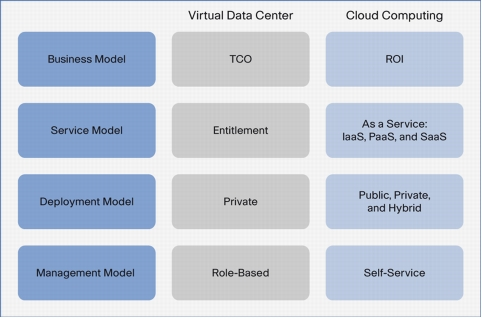
\includegraphics[width=0.91\textwidth]{white_paper.jpg}
\caption[Diferencia Entre Cloud y Datacenter]{Diferencias entre Cloud Computing y Datacenter}
\end{figure}\par

Es también muy importante notar que los datacenters tradicionales son hechos principalmente para 
aplicaciones del tipo cliente servidor. Estas aplicaciones dependen de un solo sistema operativo y 
esto se opone a las aplicaciones de la nube las cuales son construidas alrededor de una arquitectura
orientada a los servicios. Por lo tanto para ser verdaderas plataformas en la nube se debería de 
reescribir dichas aplicaciones, lo cual es imposible para la mayoría de ellas. Lo cual lleva a que
lo mas cercano que podremos estar es automatizar y orquestar nuestro ambiente, desarrollar estándares
y procesos que nos permitan escalar mas rápidamente.

Por ejemplo hoy en día todavía se administra manualmente a las VMs\footnote{Virtual Machines}. El 
problemas radica en que las organizaciones deben lidiar con un mayor numero de maquinas virtuales.
Para solucionar el problema se contratan mas cantidad de administradores, lo cual es bueno para la 
economía, pero no permite escalar de la manera mas óptima posible, con lo cual se debe aprender a
construir estándares, automatizar y orquestar con el fin de mantenerse lo mas alejado posible de
las tareas manuales repetitivas, las cuales consumen muchos recursos humanos.

Otra diferencia significativa entre cloud y datacenters es que uno de estos últimos el negocio 
depende completamente en el departamento de IT para adquirir los recursos necesarios, lo cual es que
no exista un acercamiento de auto-servicio o siquiera un acercamiento a algo orientado a los 
servicios. Básicamente existe un ``mozo" de IT que toma los requerimientos, construye manualmente una
VM que cumple con los susodichos requerimientos y luego se la entrega a los dueños de las 
aplicaciones.

En un modelo de nube, se tiene un portal de auto-servicio con maquina virtuales predefinidas 
ofreciendo lo que los dueños de las aplicaciones pueden consumir y ellos deben construir las 
aplicaciones para que se puedan desempeñar en los frameworks predefinidos. 

También se puede llevar un paso mas adelante al crear el concepto de servicios. En este caso el 
servicio es una colección de VMs que son manejadas por una sola entidad; VMware vSphere y Citrix 
XnServer llaman a este concepto vApps. Cuando esto se aplica al diseño cloud, se termina ofreciendo
servicios que los usuarios pueden consumir o aprovisionarlos.

Finalmente se podría decir que cuando se construye un cloud la infraestructura queda altamente 
automatizada y orquestada. Como resultado la forma tradicional de acoplar mas racks e instalarlos 
cambia a favor de servers sin cambio que despliegan la imagen correcta dependiendo de la dirección IP
de la que se están conectando.

\section{Conclusiones}

\newpage

\begin{thebibliography}{1}

\bibitem{caractCC}		
\emph{Caracteristicas de las aplicaciones. }
 21 Abr 2013\\
\url{http://www.societic.com/2010/03/cloud-computing-caracteristicas-de\\-las-aplicaciones-en-cloud/}
 
\bibitem{ieeeCC} 
\emph{La nube es la computadora. } 
 21 Abr 2013\\
 \url{http://spectrum.ieee.org/computing/hardware/the-cloud-is-the-computer}

\bibitem{AEC2}
\emph{Amazon EC2. }
 25 May 2013\\
 \url{http://aws.amazon.com/es/ec2/} 

\bibitem{paas}
\emph{Enterprise Cloud Curves Ahead, PaaS Carefully. }
 26 May 2013\\
 \url{http://www.cloudtweaks.com/2012/03/enterprise-cloud-curves-ahead-paas-carefully/}

\bibitem{csa}
\emph{Guía para la seguridad en áreas criticas de atención en Cloud Computing. } Cloud Security 
Alliance,
 USA, Nov 2009.

\bibitem{dataCCC}
	Lori MacVittie	
	\emph{Cloud Computing versus Cloud Data Centers.} DevCentral,
	USA,
	Sep 2009. 	

\end{thebibliography}

\end{document}
